\bookchapter{第四十二章：大規模モデルの全景とAPI実践}

\chapterintro{ここ数章は「AIとどう協働するか」の話でしたが、本章ではもっと基本的な問題を扱います：「どのAIを使う？どう使う？」2026年8月の大規模モデルの情勢は、すでに非常に豊かです——世界ではGPT、Claude、Geminiの三強が争い、中国ではDeepSeek、通義千問（Qwen）、GLM、Kimi、豆包（Doubao）が百花繚乱です。どのモデルにもそれぞれの性格と得意分野があります：選択が合っていれば仕事ははかどり、合っていなければ労多くして功少なしです。本章ではこれらのモデルを紹介するだけでなく、APIを通じて自分のアプリに組み込む方法、そして自分のニーズに合ったTokenプラン（用量プラン）の選び方も教えます。}

\booksection{一、世界の主流大モデル：三強の構図}

2026年8月の世界の大モデル市場では、OpenAI（GPTシリーズ）、Anthropic（Claudeシリーズ）、Google（Geminiシリーズ）の三強が並び立つ構図ができています。どこも個性ははっきりしています——ひとつずつ見ていきましょう。

\booksubsection{OpenAI GPT-5.6シリーズ：万能でバランスの取れたオールラウンダー}

OpenAIは大モデルの波の火付け役で、GPTシリーズは今も世界で最も広く使われているモデルです。2026年7月にリリースされたGPT-5.6シリーズは、三段階の位置づけを採用しています：フラッグシップのGPT-5.6 Solは高度な推論ニーズ向け、バランス型のGPT-5.6 Terraは日々の開発向け、軽量のGPT-5.6 Lunaは高い同時処理と低コストの場面向けです。3モデルとも105万Tokenのコンテキストウィンドウを共有し、画像入力、関数呼び出し、構造化出力に対応しています。

\begin{center}
\begin{tabularx}{\linewidth}{|X|X|X|X|X|}
\hline
\textbf{モデル} & \textbf{位置づけ} & \textbf{入力（/100万Token）} & \textbf{出力（/100万Token）} & \textbf{コンテキストウィンドウ} \tabularnewline
\hline
GPT-5.6 Sol & フラッグシップ推論 & US\$5.00（約36元） & US\$30.00（約217元） & 105万トークン \tabularnewline
GPT-5.6 Terra & バランス·日常 & US\$2.50（約18元） & US\$15.00（約109元） & 105万トークン \tabularnewline
GPT-5.6 Luna & 軽量·低コスト & US\$1.00（約7元） & US\$6.00（約44元） & 105万トークン \tabularnewline
\hline
\end{tabularx}
\end{center}

\begin{center}\small\color{gray}OpenAI GPT-5.6シリーズの料金（2026年8月）\end{center}

GPTシリーズの中核的な強みは「バランス」——推論、プログラミング、ライティング、マルチモーダルと、目立つ弱みがありません。OpenAIの巨大なプラグインエコシステムと開発者コミュニティもあり、対応ドキュメントとツールチェーンが最も整っています。「何を選べばいいかわからない」という場面では、GPTは「目をつぶって選んでも間違いない」デフォルトの答えです。ただし弱みもあります：中国国内からのアクセスには特殊なネット環境が必要で、中国語の表現にはときどき「翻訳くささ」があり、API価格は中〜高水準です。

\textbf{良いニュース}\par

OpenAIは2026年8月、無料ユーザーのデフォルトモデルをGPT-5.6 Lunaに引き上げ、テキストチャットを無制限に開放すると発表しました。つまりGPTの基本能力をコストゼロで体験でき、より強い推論やAPI呼び出しが必要なときにだけ支払えばよいのです。

\booksubsection{Anthropic Claudeシリーズ：プログラミングと厳密さの頂点}

GPTがオールラウンダーなら、Claudeはプログラミング分野の「頂点」です。AnthropicのClaudeシリーズはSWE-bench（ソフトウェアエンジニアリングのベンチマーク）で長期間にわたり大差をつけて首位を保ち、コード生成の質と、エンジニアリングレベルのプロジェクトを形にする力は業界トップです。さらに貴重なのは、Claudeのハルシネーション率（でたらめな情報を生成する確率）が業界最低の約1\%であること——学術や法務など、高精度が求められる場面に特に適しています。

Claudeのもうひとつの切り札は超長いコンテキスト：100万Tokenのコンテキストウィンドウに対応し、何百ページもの契約書やコードベース全体を、細部を見落とさず一気に「読み切る」ことができます。これはコードのリファクタリングや長文書の分析などの場面で、ほぼ代替がききません。ターミナルAIプログラミングツールのClaude Codeは、2026年半ばには年間換算収益25億米ドルに達しています——これが、Claudeのプログラミング能力が最も認められている証拠です。

\begin{center}
\begin{tabularx}{\linewidth}{|X|X|X|X|X|}
\hline
\textbf{モデル} & \textbf{位置づけ} & \textbf{入力（/100万Token）} & \textbf{出力（/100万Token）} & \textbf{コンテキストウィンドウ} \tabularnewline
\hline
Claude Fable 5 & フラッグシップ & US\$10.00（約72元） & US\$50.00（約362元） & 100万トークン \tabularnewline
Claude Opus 4.8 & プロ向け & US\$5.00（約36元） & US\$25.00（約181元） & 100万トークン \tabularnewline
Claude Sonnet 5 & コスパ重視 & US\$2.00（約14元） & US\$10.00（約72元） & 100万トークン \tabularnewline
\hline
\end{tabularx}
\end{center}

\begin{center}\small\color{gray}Anthropic Claudeシリーズの料金（2026年8月、Sonnet 5は優遇価格）\end{center}

Claudeの弱みは価格です——Fable 5の出力価格は全モデル中で最も高く、100万Tokenあたり50米ドル。マルチモーダル対応（画像·動画の理解）もやや弱めです。予算の限られた個人開発者には、優遇期間中のSonnet 5のコストパフォーマンスがとても際立っています。

\booksubsection{Google Geminiシリーズ：マルチモーダルの王者}

GoogleのGeminiシリーズは2026年にバージョン3.1 Proまで進化しました。Gemini最大の切り札はネイティブマルチモーダル——画像とテキストの解析は正確で、OCRの表認識にミスがなく、動画フレームの抽出も効率的、さらに音声·動画の深い解析にも対応します。Googleエコシステム（検索、メール、クラウドサービス）と深く結びついており、リアルタイムの情報検索とモーダルをまたいだ理解で際立った強さを発揮します。Geminiは200万Tokenの超長いコンテキスト入力にも対応しており、現時点で最も大きなコンテキストウィンドウを持つモデルです。

Geminiの位置づけは「科学的推論とマルチモーダルの場面での第一選択」です。プロジェクトに大量の画像分析、動画の理解、科学計算が関わるなら、Geminiにはほぼ対抗馬がいません。ただし、テキストだけのコード生成ではClaudeに少し劣り、中国語の表現も中国国産モデルほど自然ではありません。

\begin{center}
\begin{tabularx}{\linewidth}{|X|X|X|X|}
\hline
\textbf{比較項目} & \textbf{GPT-5.6} & \textbf{Claude Fable 5} & \textbf{Gemini 3.1 Pro} \tabularnewline
\hline
総合スコア & 94.8 & 95.0 & 92.1 \tabularnewline
コーディング力（SWE-bench） & 74.9\% & 64.3\% (Pro) & 中程度 \tabularnewline
コンテキストウィンドウ & 105万トークン & 100万トークン & 200万トークン \tabularnewline
マルチモーダル能力 & バランス & やや弱い & 最強 \tabularnewline
ハルシネーション率 & 低め & 最低（約1\%） & 低め \tabularnewline
中国国内での利用可否 & 特殊なネット環境が必要 & 特殊なネット環境が必要 & 特殊なネット環境が必要 \tabularnewline
APIエコシステム & 最も整っている & 成長中 & Googleエコシステムとの一体化 \tabularnewline
\hline
\end{tabularx}
\end{center}

\begin{center}\small\color{gray}国際三大モデルの横断比較（2026年8月）\end{center}

\begin{tcbwarn}{注意：中国国内で使うときの現実的なハードル}
中国国内の開発者にとって、GPT、Claude、Geminiの最大の障害はネットワークアクセスです。AzureのプロキシやAPI集約プラットフォームなどを通じて間接的に利用することもできますが、安定性と法令遵守については、自分で評価する必要があります。データの安全に厳しい要件があるプロジェクトでは、まず中国国産モデルの利用をおすすめします。

\end{tcbwarn}

\booksection{二、中国国産の主流大モデル：百花繚乱}

2026年の中国国産大モデルは、「追いかける側」から「並んで走る側」になり、分野によっては「先頭を走る側」にまで成長しました。2023年の「中身の流用」騒動とは違い、2026年の国産フラッグシップモデルは、論理推論、コード生成、中国語理解などの面で世界トップクラスのモデルとほぼ互角になり、差は5\%以内まで縮まっています。さらに大事なのは、中国語の場面、価格、コンプライアンスを満たした運用では、国産モデルに代えられない強みがあることです。

\booksubsection{DeepSeek V4：コストパフォーマンスの王者}

DeepSeek（深度求索）は中国国産大モデルの中で現象級の存在です。2025年の初め、DeepSeek-V3は「GPTより10分の1安いのに能力は同等」という位置づけで市場を震撼させ、業界では「汎用AI大モデルの斬殺ライン」と呼ばれました——それより安いものは使い勝手で及ばず、それより高いものはコストの安さと提供力で及ばない、という意味です。2026年8月にはDeepSeek V4正式版が登場しました：1.6兆パラメータのMoEアーキテクチャ、動かすのは約49B、100万Tokenの劣化なしコンテキストに対応し、コードのコストパフォーマンスは世界の天井と広く見られています。

DeepSeek V4はAgent能力で大きく跳ね上がりました——DeepSWEベンチマークが12.8から62.7へ（+390\%）、NL2Repoが38.5から61.5へ。APIにはResponses APIとAnthropic APIの二つのプロトコル対応が新たに加わり、CodexやClaude Codeといった主流のプログラミングツールとの互換性が実現しています。つまり、ClaudeのAPIの代わりにDeepSeekのAPIを使ってClaude Codeを動かせる——コストは数分の一に下がり、体験はほぼ同じです。

\begin{center}
\begin{tabularx}{\linewidth}{|X|X|X|X|X|}
\hline
\textbf{モデル} & \textbf{位置づけ} & \textbf{入力（/100万Token）} & \textbf{出力（/100万Token）} & \textbf{コンテキストウィンドウ} \tabularnewline
\hline
DeepSeek V4 Pro & フラッグシップ推論 & 3元（約US\$0.43） & 6元（約US\$0.87） & 100万トークン \tabularnewline
DeepSeek V4 Flash & 軽量·高速 & 1元（約US\$0.14） & 2元（約US\$0.28） & 100万トークン \tabularnewline
\hline
\end{tabularx}
\end{center}

\begin{center}\small\color{gray}DeepSeek V4シリーズの料金（2026年8月、セール価格）\end{center}

価格比較：同じく100万Tokenの入力＋100万Tokenの出力で、DeepSeek V4 Flashは約0.42米ドル、GPT-5.6 Solは約35米ドル、Claude Fable 5は約60米ドル。差はなんと80〜140倍にもなります。

\textbf{落とし穴に注意：DeepSeekは値上げの予定です}\par

DeepSeek公式は2026年8月6日、「近いうちにAPI料金を大幅に引き上げる計画」と発表しており、セール価格は長くは続かない可能性があります。一部のメディアでは値上げ幅が30倍に達する可能性があると報じられていますが、8月14日時点で公式は最終的な改定案を公表していません。さらにDeepSeek V4正式版では、ピーク·オフピーク料金の仕組みが導入され——ピーク時間帯のAPI呼び出し料金はそのまま2倍になります。最新の料金は公式の発表を確認することをおすすめします。

\booksubsection{通義千問 Qwen3.7 Max：アリババクラウドのエンタープライズ向け選択肢}

アリババクラウドの通義千問（Qwen）シリーズは、アリババクラウドのエコシステムを背景に、企業向けの運用で元から強みを持っています。2026年7月のQwen3.7 Maxが現行のフラッグシップ：235Bパラメータのデンスモデルで、ネイティブコンテキストは256K、1Mまで拡張可能です。Qwenの中核的な強みは：成熟したオープンソースエコシステム（7Bから235Bまで全シリーズがオープンソース）、正確な中国語の場面の理解、アリババクラウド基盤との深い統合です。

\begin{center}
\begin{tabularx}{\linewidth}{|X|X|X|}
\hline
\textbf{モデル} & \textbf{出力価格（/100万Token）} & \textbf{向いている場面} \tabularnewline
\hline
qwen-turbo & 0.6元 & ごくシンプルな質疑応答、テキスト分類、高負荷な同時処理 \tabularnewline
qwen-long & 2.0元 & 10Mの超長コンテキスト処理 \tabularnewline
qwen3.7-flash & 7.2元 & 汎用対話、コンテンツ生成 \tabularnewline
qwen3.7-plus & 12.0元 & マルチモーダル（画像＋動画）、中国語創作 \tabularnewline
qwen3.7-max & 36.0元 & フラッグシップの中国語能力、複雑なタスク \tabularnewline
\hline
\end{tabularx}
\end{center}

\begin{center}\small\color{gray}Qwen（通義千問）シリーズの段階制料金（2026年8月）\end{center}

Qwenの料金は段階制を採用しています。極めて低コストのqwen-turbo（出力0.6元/100万トークン）から、フラッグシップのqwen3.7-max（出力36元/100万トークン）まで、軽量な質疑応答から複雑な推論まで、あらゆるシーンのニーズをカバーします。すでにAlibaba Cloudを使っている企業にとって、Qwenは最も手軽な統合の選択肢です。

\booksubsection{智譜GLM-5.1：国産SWE-bench第1位}

智譜AI（Zhipu AI）のGLMシリーズは2026年に目覚ましい活躍を見せています。GLM-5.1はSWE-benchで国産第1位の成績を獲得しました。744BのMoE（混合エキスパート）ハイブリッドアーキテクチャで、100万トークンのコンテキストに対応します。特徴は中国語の意味理解が正確なこと、そして中国国内のコンプライアンス準拠のプライベート導入に対応していることです。これはデータセキュリティへの要求が厳しい金融·行政の場面でとても重要になります。GLM-5.1の料金は入力6元、出力24元/100万トークンで、国産モデルの中堅クラスです。

\booksubsection{Kimi K3：超長文の王}

Moonshot AI（月の暗面）のKimiシリーズは、超長文の処理能力で知られています。2026年7月に公開されたKimi K3は2.8兆パラメータの規模を誇り、複数の難しいタスクの評価で世界の第一集団に入りました。Kimiの主戦場は、大きなコードベースの分析や長文ドキュメントの検索拡張です。本1冊分のテキストも、プロジェクト一式のコードも処理でき、「needle in a haystack（干し草の山から針探し）」式の検索タスクで優れた成績を収めます。Kimiの料金は比較的高め（出力約12〜20元/100万トークン）ですが、長文ユースケースでのコストパフォーマンスには他の追随を許しません。

\booksubsection{豆包（Doubao）：ByteDanceのオールラウンダー}

ByteDanceの豆包（Doubao）シリーズは2026年も安定したパフォーマンスを見せています。Doubao Seed 2.1 Proは火山引擎（Volcano Engine）のフラッグシップモデルで、256Kのコンテキストを持ち、実測でも総合的に安定した動きを見せ、中国語のユースケースでの体験が特に優れています。豆包の強みは、登録するだけで大量の無料トークンがもらえること、火山引擎エコシステムとの統合が整っていること、そして料金が中国国内で最安クラスのひとつであることです。手早くAIプログラミングを体験してみたい初心者には、豆包がハードルゼロの入門向け選択肢です。

\begin{center}
\begin{tabularx}{\linewidth}{|X|X|X|X|X|X|}
\hline
\textbf{比較項目} & \textbf{DeepSeek V4} & \textbf{Qwen3.7 Max} & \textbf{GLM-5.1} & \textbf{Kimi K3} & \textbf{Doubao 2.1 Pro} \tabularnewline
\hline
総合スコア & 87.5 & 89.7 & 90.5 & 88+ & 85+ \tabularnewline
プログラミング能力 & 極めて強力 & 強 & 国産SWE第1位 & 強 & 中の上 \tabularnewline
中国語理解 & 優秀 & 優秀 & 正確 & 優秀 & 優秀 \tabularnewline
コンテキストウィンドウ & 100万 & 256K-1M & 100万 & 超長文 & 256K \tabularnewline
出力価格（元/100万トークン） & 6 & 36 & 24 & 12-20 & 30 \tabularnewline
オープンソース & MITライセンス & 全シリーズ公開 & 一部公開 & クローズドソース & クローズドソース \tabularnewline
プライベート導入 & 対応 & 対応 & 対応 & 非対応 & 非対応 \tabularnewline
\hline
\end{tabularx}
\end{center}

\begin{center}\small\color{gray}国産5大モデルの横断比較（2026年8月）\end{center}

重要なトレンドがひとつあります。国産モデルとGPT/Claudeの間に感じられた「世代の差」が、もう消えたということです。論理推論や数学コンテストでは、国産フラッグシップとGPT-5のスコア差はほぼ一桁です。体系立ったアーキテクチャ思考や複雑なエンジニアリング推論では、Claudeが依然リードしています。より「ひらめき」のあるアーキテクチャ案を出せる一方で、国産モデルはときどき「マニュアル通り」に見えます。ただし、中国語のユースケース、コスト管理、コンプライアンス対応の導入では、国産モデルが圧倒的な優位に立ちます。

\begin{center}
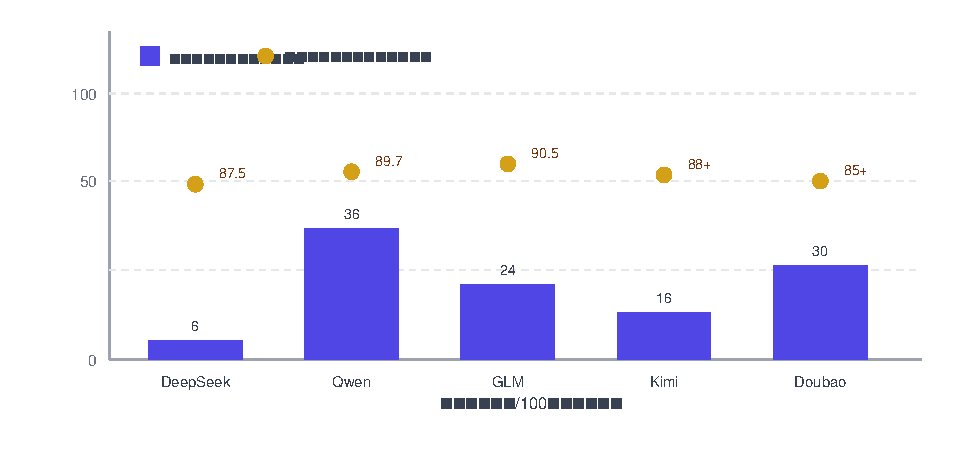
\includegraphics[width=0.92\linewidth]{figures/fig-di-si-shi-er-zhang-1}
\\[2pt]\small 図4：5モデルの価格と性能の比較（価格は低いほど、スコアは高いほど良い）
\end{center}

\booksection{三、モデル選択の意思決定フレームワーク}

各モデルの特徴がわかったところで、自分のプロジェクトにはどのモデルを選べばいいのでしょうか。ここで「四問決定法」をお渡しします。4つの質問に答えるだけで、あなたに最も合ったモデルを絞り込めます。

プロジェクトは国内向けですか、国際展開ですか？

国内 国産モデルを選ぶ

|

国際 海外モデルも選べる

中心の仕事はプログラミングですか、それとも別？

プログラミング Claude または DeepSeek

|

その他 判断を続ける

超長コンテキスト（>50万トークン）が必要？

必要 Gemini または Kimi

|

不要 判断を続ける

予算は厳しい？

センシティブ DeepSeek または Qwen-turbo

|

非センシティブ GPT-5.6 または Claude

\begin{center}\small\color{gray}図5：大規模モデル選択の四問決定法\end{center}

\begin{tcbinfo}{ワンポイント：組み合わせ戦略}
この決定法は金科玉条ではありません。多くの場面では、複数のモデルを組み合わせて使う必要があります。よくある組み合わせ戦略はこうです。日常の開発にはDeepSeekかQwen（コストが低く中国語が得意）、重要なアーキテクチャ設計にはClaude（推論が強くハルシネーションが少ない）、マルチモーダル分析にはGemini（画像·動画の処理）。「1つのモデルを使い倒す」のではなく、必要に応じてモデルを切り替えましょう。

\end{tcbinfo}

\booksection{四、API呼び出し入門：ゼロから大規模モデルにつなぐ}

多くのAIプログラミング解説は対話画面の使い方しか教えてくれませんが、本物の「AIプログラミング」——自分のアプリから大規模モデルを呼び出すこと——にはAPIが必要です。API（Application Programming Interface、アプリケーションプログラミングインターフェース）はプログラム同士の通信プロトコルです。APIを通れば、あなたのコードは関数を1つ呼び出すように大規模モデルの能力を利用できます。

\booksubsection{トークンとは}

APIを理解する前に、まず「トークン（Token）」という概念を押さえる必要があります。トークンは大規模モデルの課金の基本単位で、「AIにとっての読み書きの単位」と考えるとよいでしょう。1トークンはおよそ、英語では0.75単語（4文字）、中国語では0.5〜1文字に対応します。中国語1000字のテキストなら、約1500〜2000トークンを消費します。

トークンは字数でも文字数でもありません。大規模モデルは専用のトークナイザー（Tokenizer）でテキストをトークンに分割します。同じ語でもモデルによってトークン数は異なることがあります。たとえば「人工智能（人工知能）」はGPTでは3トークン、DeepSeekでは2トークンになる、といった具合です。ほとんどのモデルのAPIは実際に消費したトークン数を返すので、APIレスポンスで確認できます。

\begin{tcbinfo}{トークンコストのクイック見積もり}
中国語100万字は約150万トークンに相当します。DeepSeek V4 Flashで入力100万字＋出力100万字を処理すると、コストは約0.42米ドル（約3元）。同じ量をClaude Fable 5で処理すると、約60米ドル（約434元）かかります。モデル選びがプロジェクトのコストを直接左右するのはこのためです。

\end{tcbinfo}

\booksubsection{APIキーの取得}

大規模モデルAPIを使う最初のステップはAPIキーの取得です。認証に使う一連の文字列のことですね。各モデル提供元にはそれぞれAPIプラットフォームがあり、アカウントを登録してAPIキーを作成する必要があります。主なモデルのAPIプラットフォームへの入り口と取得手順は以下のとおりです。

\begin{center}
\begin{tabularx}{\linewidth}{|X|X|X|X|}
\hline
\textbf{モデル} & \textbf{APIプラットフォーム} & \textbf{取得手順} & \textbf{無料枠} \tabularnewline
\hline
DeepSeek & platform.deepseek.com & 登録 実名認証 APIキー作成 & 新規ユーザーに利用枠を進呈 \tabularnewline
Qwen（通義千問） & bailian.aliyun.com（百煉プラットフォーム） & Alibaba Cloudアカウントでログイン サービスを有効化 キーを作成 & 新規ユーザーは無料トライアル付き \tabularnewline
智譜GLM & open.bigmodel.cn & 登録 実名認証 APIキー作成 & 新規ユーザーに利用枠を進呈 \tabularnewline
Kimi & platform.moonshot.cn & 登録 実名認証 APIキー作成 & 限定的な無料枠 \tabularnewline
豆包（Doubao） & volcengine.com（Volcengine） & 登録 方舟（Ark）を有効化 APIキー作成 & 登録で大量のトークンをプレゼント \tabularnewline
OpenAI GPT & platform.openai.com & 登録 クレジットカード登録 APIキー作成 & 無料枠なし（有料） \tabularnewline
Anthropic Claude & console.anthropic.com & 登録 カード登録 APIキー作成 & 新規ユーザーに少額の利用枠 \tabularnewline
\hline
\end{tabularx}
\end{center}

\begin{center}\small\color{gray}主なモデルのAPIプラットフォームとキー取得方法（2026年8月）\end{center}

\textbf{安全上の注意：APIキー＝財布のパスワード}\par

APIキーはあなたの財布のパスワードと同じです。キーを手にした人は誰でも、あなたの利用枠でモデルを呼び出せてしまいます。したがって、APIキーをコードに書かない（環境変数で管理する）、キーを含むコードを公開Gitリポジトリにコミットしない、キーが映ったスクリーンショットをSNSに共有しない——この3つは絶対に守ってください。キーが漏れた場合は、すぐにプラットフォームで削除して作り直しましょう。

\booksubsection{初めてのAPI呼び出し}

APIキーを取得すれば、どんなプログラミング言語でも大規模モデルAPIを呼び出せます。以下ではPythonで最もシンプルな呼び出しをデモします。DeepSeekにメッセージを1つ送り、返信を取得します。

\begin{lstlisting}[language=Python]
# SDKのインストール：pip install openai
# DeepSeekはOpenAI SDK形式と互換あり、そのまま使える
from openai import OpenAI
import os

# 1. クライアントを作成（API Keyは環境変数から読み込む）
client = OpenAI(
    api_key=os.environ.get("DEEPSEEK_API_KEY"),
    base_url="https://api.deepseek.com"
)

# 2. リクエスト送信
response = client.chat.completions.create(
    model="deepseek-chat",  # モデル指定
    messages=[
        {"role": "system", "content": "あなたはPythonプログラミングの助手です。"},
        {"role": "user", "content": "クイックソートの関数を書いてください。"}
    ]
)

# 3. 返答を取得
print(response.choices[0].message.content)

# 4. トークン消費を確認
print(f"入力トークン: {response.usage.prompt_tokens}")
print(f"出力トークン: {response.usage.completion_tokens}")
print(f"合計トークン: {response.usage.total_tokens}")
\end{lstlisting}

このコードの核となるロジックは次のとおりです。クライアントを作成し（APIキーとモデルのアドレスを渡す） メッセージリストを組み立てる（systemが役割を設定し、userがユーザー入力） リクエストを送る 返信を受け取る。このパターンは、OpenAI形式に互換するほぼすべてのモデルに使えます。api\_keyとbase\_urlを差し替えるだけでモデルを切り替えられます。多くの国産モデルがOpenAI SDK互換形式を選ぶのはこのためです。開発者は2行変えるだけでモデルを乗り換えられ、移行コストが極めて低くて済みます。

以下は他のモデルへ切り替えるときのコードの差分です。変更が必要なのはわずか2行であることに注目してください。

\begin{lstlisting}[language=Python]
# DeepSeek
client = OpenAI(
    api_key=os.environ.get("DEEPSEEK_API_KEY"),
    base_url="https://api.deepseek.com"
)
# model="deepseek-chat"

# Qwen（百煉プラットフォーム）
client = OpenAI(
    api_key=os.environ.get("DASHSCOPE_API_KEY"),
    base_url="https://dashscope.aliyuncs.com/compatible-mode/v1"
)
# model="qwen-plus"

# Zhipu GLM
client = OpenAI(
    api_key=os.environ.get("GLM_API_KEY"),
    base_url="https://open.bigmodel.cn/api/paas/v4"
)
# model="glm-4"

# OpenAI GPT
client = OpenAI(
    api_key=os.environ.get("OPENAI_API_KEY"),
    # base_urlはデフォルトのままでOK
)
# model="gpt-5.6-terra"
\end{lstlisting}

\booksubsection{ストリーミング応答の処理}

実際のアプリでは、AIが全部書き終わるのを待って一度に表示させるのは避けたいものです。ユーザーを長く待たせてしまうからです。ストリーミング応答（Streaming）なら、AIが生成しているのと並行して一文字ずつ表示でき、ユーザー体験が大きく向上します。タイプライターのように文字がひとつずつ飛び出してくるのを見ると、体感はまったく違います。

\begin{lstlisting}[language=Python]
# ストリーミング応答：一文字ずつ出力
stream = client.chat.completions.create(
    model="deepseek-chat",
    messages=[
        {"role": "user", "content": "Pythonのバブルソートの解説を書いてください"}
    ],
    stream=True  # ストリーミングを有効化
)

# ひとかたまりずつ受け取って表示
for chunk in stream:
    if chunk.choices[0].delta.content is not None:
        print(chunk.choices[0].delta.content, end="", flush=True)
# 出力はタイプライターのように一文字ずつ流れる
\end{lstlisting}

\booksection{五、Tokenプラン購入ガイド}

ほとんどのモデル提供元には2つの課金方式があります。従量課金（Pay-as-you-go）と、定額サブスクリプション（Tokenプラン／Subscription）です。この2つの違いを理解すれば、利用コストを大幅に下げられます。

\booksubsection{従量課金 vs サブスクリプション}

\begin{center}
\begin{tabularx}{\linewidth}{|X|X|X|}
\hline
\textbf{観点} & \textbf{従量課金（Pay-as-you-go）} & \textbf{サブスクリプション（Subscription）} \tabularnewline
\hline
課金方式 & 使ったトークン分だけ支払う & 定額を前払いして利用枠を取得 \tabularnewline
向いている場面 & 利用量が不安定、たまに呼び出す程度 & 利用量が安定、高頻度で呼び出す \tabularnewline
価格面のメリット & 標準価格 & 従量課金より20〜50\%安い \tabularnewline
柔軟性 & いつでも利用でき、縛りなし & 前払いが必要で、期限切れの利用枠は失効する場合も \tabularnewline
超過時の扱い & 自動的に従量課金 & 利用枠を超えると従量課金に切り替わり \tabularnewline
代表プラットフォーム & 各モデルの公式APIプラットフォーム & OpenAI Plus/Pro, Claude Pro, Cursor Pro \tabularnewline
\hline
\end{tabularx}
\end{center}

\begin{center}\small\color{gray}2つの課金方式の比較\end{center}

初心者はまず従量課金から始めるのがおすすめです。前払いが不要で、使った分だけ払えばよいからです。月の使用量が一定の水準で安定してきたら（たとえば月50元を超えるなど）、より安い単価を得るためにサブスクリプションへの切り替えを検討しましょう。

\booksubsection{主なサブスクリプションプラン一覧}

\begin{center}
\begin{tabularx}{\linewidth}{|X|X|X|X|}
\hline
\textbf{プラン} & \textbf{月額} & \textbf{含まれる内容} & \textbf{向いている人} \tabularnewline
\hline
ChatGPT Free & 無料 & GPT-5.6 Lunaでテキスト対話し放題 & 初心者の体験用 \tabularnewline
ChatGPT Plus & US\$20/月 & GPT-5.6 Sol、画像生成、データ分析、プラグイン利用 & 中程度の利用者 \tabularnewline
ChatGPT Pro & US\$200/月 & 全モデル無制限、新機能への優先アクセス & ヘビーなプロユーザー \tabularnewline
Claude Free & 無料 & 回数制限ありのClaude対話 & 初心者の体験用 \tabularnewline
Claude Pro & US\$20/月 & Claudeを無制限に利用、新モデルへの優先アクセス & プログラミング開発者 \tabularnewline
Cursor Free & 無料 & 回数制限ありのAI補完と対話 & 初心者の体験用 \tabularnewline
Cursor Pro & US\$20/月 & AI補完し放題、月500回の高度なリクエスト & 日常的に開発する人 \tabularnewline
Cursor Business & US\$40/月/人 & チームコラボレーション、管理画面、プライバシーモード & チーム利用 \tabularnewline
\hline
\end{tabularx}
\end{center}

\begin{center}\small\color{gray}主なAIツールのサブスクリプションプラン（2026年8月）\end{center}

中国国産モデルのサブスクリプション事情は少し異なります。DeepSeekは基本的に従量課金で、月額のサブスクプランはありません。チャージしておくと、実際の使用量に応じて精算されます。Qwen（通義千問）は百煉プラットフォームで前払いのリソースパック（一定量のトークン利用枠を割引価格で購入）を提供しています。豆包も火山引擎に同様の前払いプランがあります。中国国内の開発者にとって最も経済的な組み合わせは、たいてい「DeepSeekの従量課金（日常の開発）＋豆包の無料枠（試して確認）」です。

\booksubsection{API集約プラットフォーム}

複数のモデルを同時に使いたいなら、API集約プラットフォームは手間いらずの選択肢です。集約プラットフォームは統一されたAPIキーを1つ提供し、それだけで世界中の何十種類ものモデルを呼び出せます。各プラットフォームで個別に登録する必要はありません。

\begin{center}
\begin{tabularx}{\linewidth}{|X|X|X|X|}
\hline
\textbf{プラットフォーム} & \textbf{特徴} & \textbf{価格面のメリット} & \textbf{向いている場面} \tabularnewline
\hline
OpenRouter (openrouter.ai) & 海外の集約プラットフォーム。1つのKeyで世界中のモデルを呼び出せる & 価格が透明で、リアルタイムの価格比較に対応 & 複数の海外モデルを柔軟に切り替えたい場合 \tabularnewline
SiliconFlow (siliconflow.cn) & 中国国内の集約プラットフォーム。各種国産モデルのAPIを提供 & 公式より20〜30\%安い & 中国国内の開発者、複数モデルの価格比較 \tabularnewline
Azure OpenAI（マイクロソフト経由） & マイクロソフトのAzureが仲介するOpenAI API & Batch APIなら5割引き & エンタープライズ向けOpenAI利用、大量の非同期タスク \tabularnewline
百度千帆（qianfan.baidubce.com） & 百度のAIクラウドプラットフォーム。文心（ERNIE）などのモデルを提供 & 新規ユーザーに利用枠をプレゼント & 百度エコシステムの利用者 \tabularnewline
\hline
\end{tabularx}
\end{center}

\begin{center}\small\color{gray}主なAPI集約プラットフォーム（2026年8月）\end{center}

\textbf{落とし穴注意：「共有Key」を買わない}\par

淘宝（タオバオ）や閑魚（Xianyu）などのプラットフォームで、いわゆる「共有APIキー」を買ってはいけません。こうしたキーは出所が不明なことが多く、いつアカウント停止になってもおかしくありませんし、データ漏えいのリスクもあります。APIキーは必ず公式プラットフォームか正規の集約プラットフォームから入手しましょう。

\booksubsection{コスト最適化の戦略}

適切なモデルを選ぶことは第一歩にすぎず、「お得に使う」工夫も同じくらい重要です。以下は、実践で効果が確認されたコスト最適化の戦略です。

\begin{enumerate}
  \item キャッシュヒットを活用する。多くのモデルには「キャッシュ」機能があります。リクエストに、以前処理したことのある内容（システムプロンプトなど）が含まれる場合、その部分は極めて低い価格で課金されます。DeepSeekのキャッシュヒット価格は通常価格のわずか1/60です。固定のシステムプロンプトをメッセージリストの先頭に置くと、キャッシュヒットを最大化できます。
  \item レベル別ルーティング——簡単なタスクは安いモデルに、複雑なタスクは高いモデルに振り分けます。たとえばテキスト分類にはDeepSeek V4 Flash（出力2元/100万トークン）、アーキテクチャ設計にはClaude（出力181元/100万トークン）という具合です。プロジェクト内の呼び出しの80\%は、安いモデルでまかなえます。
  \item 出力の長さを制限する。APIは出力トークンで課金されるため、出力が長いほど高くつきます。長文を必要としない場面ではmax\_tokensパラメータを設定して出力長を制限し、AIの「余計なおしゃべり」を防ぎましょう。
  \item 非リアルタイムのタスクはBatch APIを使う。即時の応答を必要としないタスク（一括データアノテーション、文書要約など）が大量にあるなら、Batch APIを使うと5割引きになります。OpenAIもAzureもこの機能を提供しています。
  \item トークン使用量をモニタリングする。ほとんどのAPIプラットフォームには使用量統計のダッシュボードがあります。定期的に使用量の内訳を確認し、トークンを最も消費している呼び出しを見つけて、そこを重点的に最適化しましょう。プロンプトを少し変えるだけ（たとえば「詳しく説明してください」を「3文で説明してください」に変える）でも、トークンを50\%節約できることがあります。
\end{enumerate}

\begin{center}
\begin{tabularx}{\linewidth}{|X|X|X|X|}
\hline
\textbf{最適化の戦略} & \textbf{節約幅} & \textbf{実施の難易度} & \textbf{説明} \tabularnewline
\hline
キャッシュヒット & 最大98\% & 低 & 固定の内容をメッセージの先頭に置く \tabularnewline
レベル別ルーティング & 50\%-80\% & 中 & 簡単なタスクは安いモデルで処理 \tabularnewline
出力の長さを制限 & 30\%-60\% & 低 & max\_tokensパラメータを設定 \tabularnewline
Batch API & 50\% & 低 & 非リアルタイムタスクはバッチ処理に \tabularnewline
プロンプトの最適化 & 20\%-50\% & 中 & プロンプトを簡潔にし、冗長さを減らす \tabularnewline
\hline
\end{tabularx}
\end{center}

\begin{center}\small\color{gray}コスト最適化の戦略と効果（2026年8月）\end{center}

\booksection{六、実践：プロジェクトに大規模モデルAPIを組み込む}

本章の締めくくりは、ひとつの完全な実践です。「AI要約ジェネレーター」を作りましょう。ユーザーが長文を入力すると、大規模モデルAPIを呼び出して要約を生成します。この実践を通じて、環境設定、API呼び出し、エラー処理、コスト管理というAPI利用の一連の流れを学べます。

\begin{lstlisting}[language=Python]
# ai_summarizer.py - AI要約ジェネレーター
import os
from openai import OpenAI

# 1. 設定（API Keyは環境変数から読み込む。ハードコード禁止）
client = OpenAI(
    api_key=os.environ.get("DEEPSEEK_API_KEY"),
    base_url="https://api.deepseek.com"
)

def summarize(text: str, max_length: int = 200) -> dict:
    """テキスト要約

    Args:
        text: 要約したい元テキスト
        max_length: 要約の最大長（トークン数）

    Returns:
        dict: 要約とトークン消費情報を含む
    """
    try:
        response = client.chat.completions.create(
            model="deepseek-chat",
            messages=[
                {
                    "role": "system",
                    "content": "あなたは要約ジェネレーターです。"
                               "ユーザーが提供したテキストを簡潔にまとめてください。"
                               "要約は3文以内で。"
                },
                {
                    "role": "user",
                    "content": f"以下のテキストを要約してください:\n\n{text}"
                }
            ],
            max_tokens=max_length,  # 出力の長さを制限
            temperature=0.3  # 温度低=より安定
        )

        return {
            "success": True,
            "summary": response.choices[0].message.content,
            "input_tokens": response.usage.prompt_tokens,
            "output_tokens": response.usage.completion_tokens,
            "total_tokens": response.usage.total_tokens
        }

    except Exception as e:
        return {
            "success": False,
            "error": str(e)
        }

# 2. 使用例
if __name__ == "__main__":
    long_text = """
    （長文をここに貼り付け...）
    """

    result = summarize(long_text)

    if result["success"]:
        print(f"要約: {result['summary']}")
        print(f"トークン消費: {result['total_tokens']}")
        # コスト概算：DeepSeek V4 Flash
        cost = result['total_tokens'] * 0.000004  # 約0.4厘/1000トークン
        print(f"概算コスト: {cost:.4f} 元")
    else:
        print(f"エラー: {result['error']}")
\end{lstlisting}

このコードには、API呼び出しのベストプラクティスがいくつか盛り込まれています。APIキーは環境変数から読み込み、コードにハードコードしない。関数にはわかりやすいドキュメントと型ヒントを付ける。max\_tokensを設定して出力長を制限する。temperatureは低め（0.3）にして、より安定した出力を得る。エラー処理を完備する。コスト追跡のためにトークン消費情報を返す。このコードをAIに書かせるときは、こうした要件を伝えればOKです。AIにはそれを実現する十分な力があります。

この章の最後の教え：モデルは「弾薬」、方法論は「戦術」。弾薬を正しく選べば戦いは楽になるが、戦術が悪ければどんな弾薬でも勝てない。各モデルの特徴とAPIの使い方を知れば「弾薬庫」は十分——ただしこの戦いをどう戦うかは、前の章で学んだ思考方法論にかかっています。

\begin{tcbpractice}{やってみよう：初めてのAPI呼び出しを動かそう}
国産モデルのプラットフォームに1つ登録しましょう（おすすめはDeepSeekか智譜。どちらも新規ユーザーに利用枠をプレゼントしてくれます）。APIキーを作成し、システムの環境変数に書き込んで（コードの中ではなく！）、先ほどの「初めてのAPI呼び出し」のコードを実行します。AIの返答が表示されたその瞬間、あなたは「AIを使う側」と「AIアプリを作る側」の境界線を越えたのです。

\end{tcbpractice}

\begin{tcbsummary}{本章のまとめ}
\begin{itemize}
  \item 国際の三強：GPT-5.6（バランス型のオールラウンダー）、Claude（プログラミング能力の頂点＋ハルシネーション率わずか1\%）、Gemini（マルチモーダルの王＋200万コンテキスト）
  \item 国産の五強：DeepSeek V4（コスパの王、値上げ公告に注意）、Qwen3.7（エンタープライズ向け）、GLM-5.1（SWE国産第1位）、Kimi K3（超長文）、豆包（無料で入門）
  \item 四問決定法：デプロイ先は？プログラミングかそれ以外か？超長文コンテキストは必要か？予算はシビアか？
  \item トークンは課金単位：中国語1文字は約1.5〜2トークン。100万字で約150万トークン
  \item APIキー＝財布のパスワード：環境変数で管理。ハードコードは絶対NG、Gitにアップロードしない
  \item 国産モデルはほぼOpenAI SDK互換：モデルの切り替えはapi\_keyとbase\_urlの2行を変えるだけ
  \item 節約の5つのコツ：キャッシュヒット、レベル別ルーティング、出力制限、Batch API、使用量モニタリング
\end{itemize}

\end{tcbsummary}
